\documentclass[../main.tex]{subfiles}
\graphicspath{{\subfix{../images/}}}
\begin{document}


%\subsection{Yolo Performance} \label{yolo_performance}

%%%%%%%%%%%%%%%%%%%%%%%%%%%%%%%%%%%%%%%%%%%%%%%%%%%%%%%%%%%%%%%%%%%%
% \subsection{Transfer Learning and Model Fine-Tuning}
% \label{sec:yolo_finetuning}
For this research, YOLOv8 was trained on a custom maritime dataset derived from sensor recordings collected aboard the Minion platform.
The dataset includes labeled examples of navigation markers, buoys, vessels, and other relevant maritime objects captured under diverse lighting conditions, sea states, and viewing angles.
Transfer learning was employed by initializing the network with weights pre-trained on a general-purpose dataset, then fine-tuning on the maritime-specific data to adapt the model to the target domain.

Fine-tuning was conducted using the Ultralytics YOLOv8 framework. \cite{ultralytics} %, employing a combination of data augmentation techniques—including random horizontal flips, exposure shifts, and image rotations—to improve robustness under varying lighting and sea-state conditions.
% Hyperparameters such as learning rate, batch size, and the number of epochs were optimized empirically to achieve stable convergence while minimizing overfitting.
To assess the tradeoff between detection accuracy and inference speed, three YOLOv8 model size variants (YOLOv8n, YOLOv8s, and YOLOv8m) were trained using the default parameters and evaluated over a set of training epochs.
Each model’s number of trainable parameters, summarized in Table~\ref{tab:yolo_variants}, corresponds to differences in backbone depth and channel width that balance model capacity against computational efficiency.
Training was performed over multiple epochs to identify the most efficient configuration for the dataset.
The YOLOv8m model exhibited no measurable improvement in mean average precision compared to YOLOv8s, while requiring substantially greater computational resources.
The YOLOv8s model achieved full convergence within approximately 80 epochs without signs of overtraining and was therefore selected for subsequent testing and deployment.

\begin{table}[htbp]
\centering
\caption{YOLOv8 model comparison for visual detection tasks.}
\begin{tabular}{l c c c c}
\hline
Model & Params (M) & FPS (RTX 3090) & mAP@50 \\
\hline
YOLOv8n & 3.2 &  110 & 0.79 \\
YOLOv8s & 11.2 &  85 & 0.84 \\
YOLOv8m & 25.9 &  63 & 0.87 \\
\hline
\end{tabular}
\label{tab:yolo_variants}
\end{table}

Inference timing was recorded using per-process timers to isolate image capture, pre-processing, neural inference, and post-processing durations.
This timing-based comparison allows fair assessment against non-GPU LiDAR pipelines in later sections.

\begin{figure}[htbp]
    \centering
    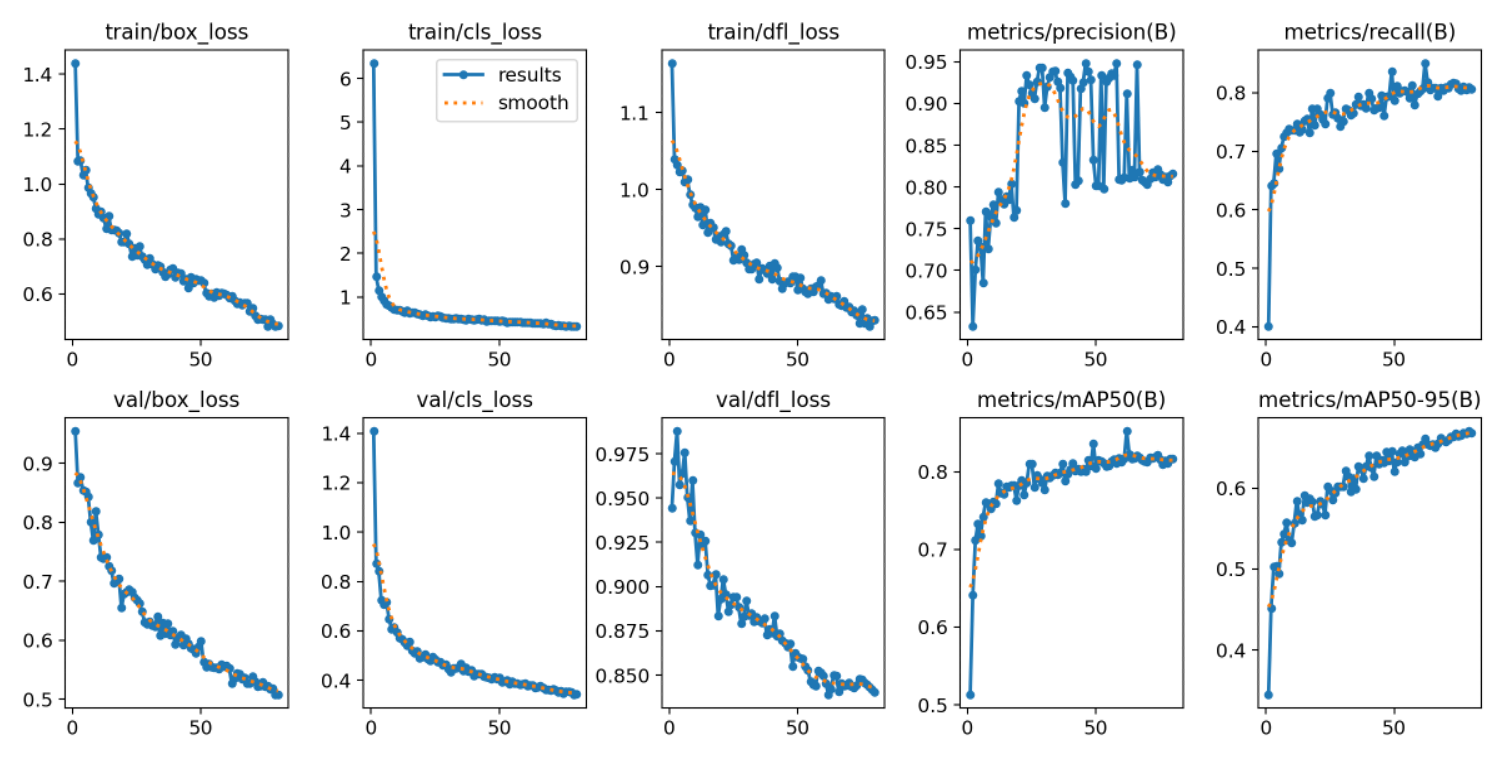
\includegraphics[width=0.85\linewidth]{Images/yolo/YOLO_training.png}
    \caption{YOLOv8 transfer learning convergence showing loss and mean Average Precision (mAP) trends over 80 epochs with the small model.}
    \label{fig:yolo_training_curve}
\end{figure}


% %%%%%%%%%%%%%%%%%%%%%%%%%%%%%%%%%%%%%%%%%%%%%%%%%%%%%%%%%%%%%%%%%%%%
% \subsection{Retraining Results and Performance Evaluation}
% \label{sec:yolo_results}



The fine-tuned YOLOv8-s model achieved the best balance of accuracy and speed for maritime operations.
Model evaluation was performed using a holdout dataset collected under variable illumination and sea states.
Performance metrics include mean Average Precision (mAP@50), precision-recall curves, and confusion matrices for key object classes such as vessels, buoys, and docks.

\begin{figure}[htbp]
    \centering
    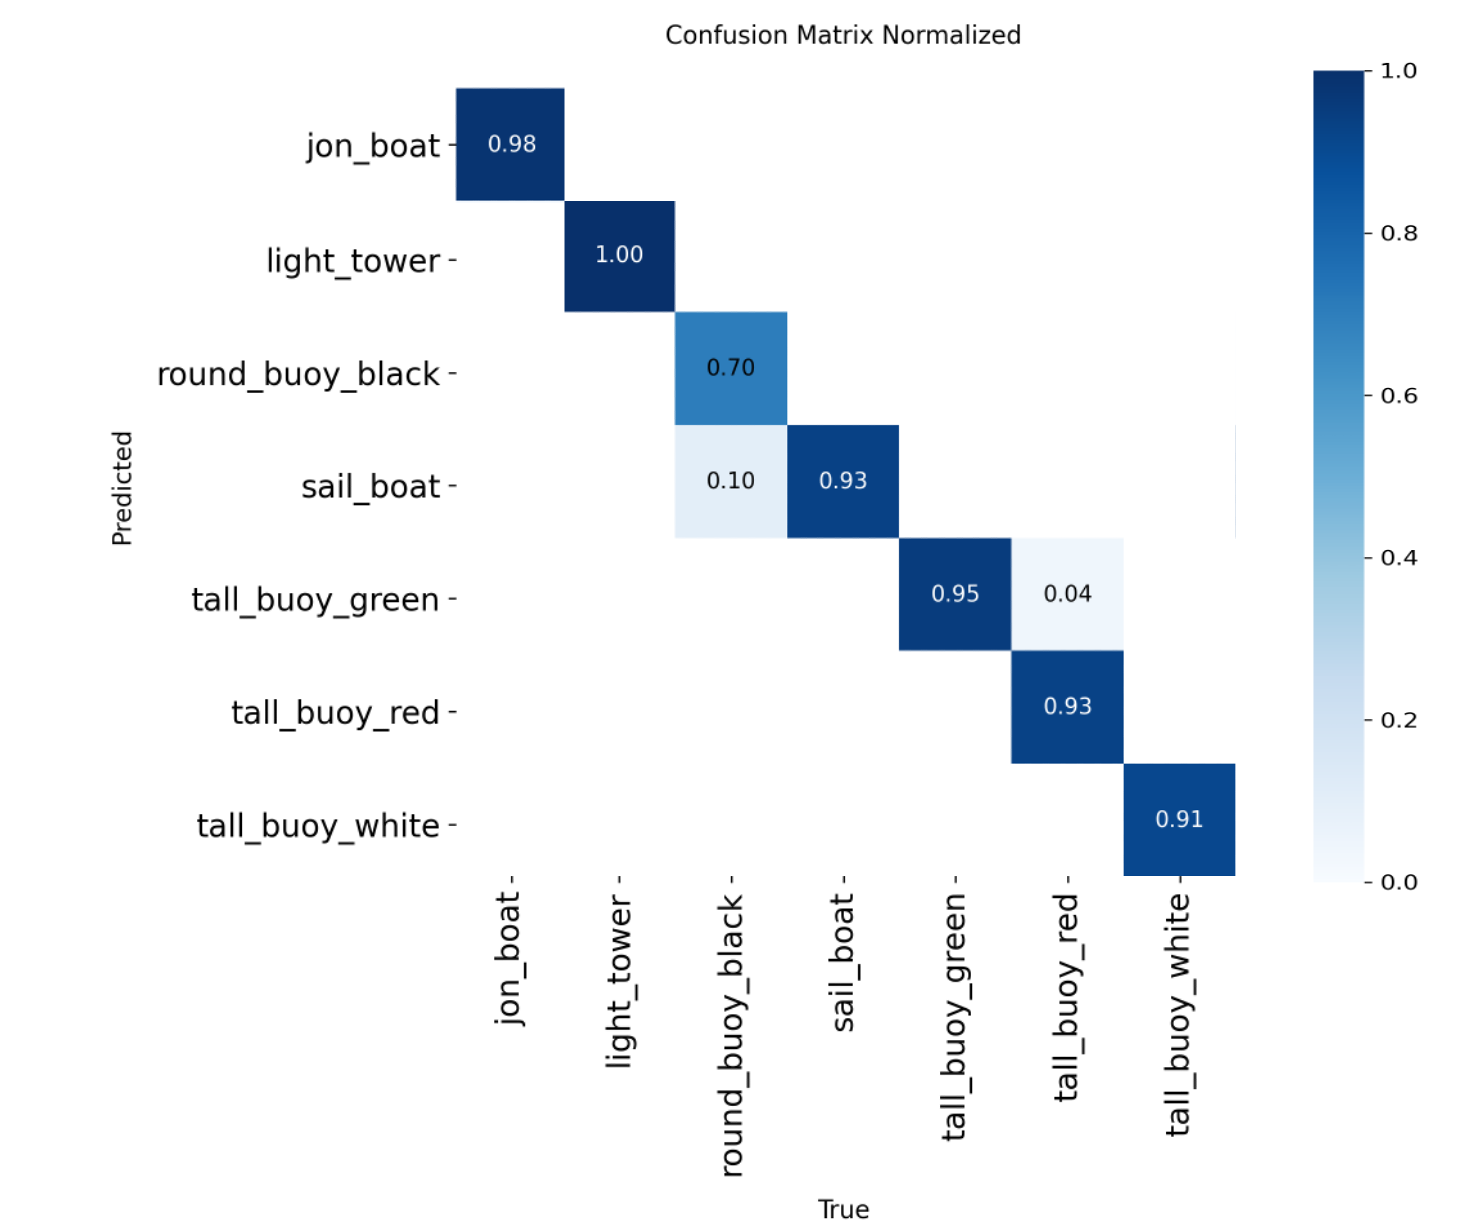
\includegraphics[width=0.8\linewidth]{Images/yolo/YOLO_training_results.png}
    \caption{Confusion matrix for YOLOv8-s model evaluated on the test dataset.}
    \label{fig:yolo_confusion_matrix}
\end{figure}

% \begin{figure}[htbp]
%     \centering
%     \includegraphics[width=0.8\linewidth]{Images/yolo_pr_curve.png}
%     \caption{Precision–recall curve for primary object classes.}
%     \label{fig:yolo_pr_curve}
% \end{figure}

Results indicate consistent detection performance across lighting conditions with minimal false positives on horizon clutter.
Retraining improved small-object detection by approximately X\% compared to baseline COCO-trained weights, confirming the benefit of domain adaptation for maritime imagery.

% %%%%%%%%%%%%%%%%%%%%%%%%%%%%%%%%%%%%%%%%%%%%%%%%%%%%%%%%%%%%%%%%%%%%
% \subsection{Discussion and Relevance to Sensor Fusion}
% \label{sec:yolo_discussion}

The fine-tuned YOLOv8 network serves as the visual baseline for comparison with LiDAR-based object detection methods presented in Section~\ref{gbcache}.
By isolating timing metrics for each processing stage, the performance comparison remains hardware-agnostic.
This approach emphasizes algorithmic latency, rather than total frame rate, as the primary metric for evaluating real-time feasibility in multi-sensor fusion.


\end{document}